	\subsection{HelloDate}
		Um zu sehen, wie die Entwicklung deiner eigenen Roboter-Software im Folgenden ablaufen wird, wirst du nun am Hello-World-Programm eine kleine Änderung durchführen und anschließend das aktualisierte Programm auf den Roboter laden.
		
		Öffne dazu zuerst die \bfcode{HelloDate.java}-Datei. Ändere den Code nun, sodass er dem folgenden Code ähnelt:\\
		\textbf{Wichtig:} Ändere in keiner Aufgabe die imports oder den Package-Namen. Diese sind bereits so wie sie sein müssen.
		
		\lstinputlisting[firstline=3]{\solpath/HelloDate.java}
		
		\begin{itemize}
		\item Die Imports von \bfcode{java.text.SimpleDateFormat} und \bfcode{java.util.Date} sind neu hinzugekommen.
		\item Außerdem gibt es nun eine Variable \bfcode{formatter} (Zeile 17), die in der Lage ist, das aktuelle Datum formatiert auszugeben (\bfcode{formatter.format(new Date())}, Zeile 19)).
		\end{itemize}
		Um die Änderungen nun auf das Handy zu übertragen, muss die App neu installiert werden.
		\begin{enumerate}
		\item Zuerst musst du deine Änderungen am Code 
		 speichern\footnote{Oben Links auf das Diskettensymbol klicken 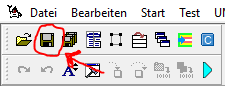
\includegraphics[]{img/je_savebutton}}. 
		\item Betätige jetzt die Schaltfläche “Starten” .
		\item Nachdem im Compiler-Fenster die Meldung “BUILD SUCCESSFUL” erschienen ist, wird auf dem Handy die Mindroid-App automatisch geschlossen und wieder geöffnet.
		\item Wähle “Verbindung zum EV3-Brick herstellen”
		\item Wähle im Dropdown “HelloWorld” aus und betätige “Start”.
		\item Auf dem Display sollte nun das aktuelle Datum ausgegeben werden.
		
		\end{enumerate}
		
	\textbf{Übrigens}\\
		
	Falls du erfahren möchtest, wie man bspw. die aktuelle Uhrzeit mithilfe von SimpleDateFormat ausgibt, klicke mit Rechts auf den Klassennamen SimpleDateFormat und wähle den Eintrag “API-Hilfe.” Im sich öffnenden Fenster findest du die Dokumentation der Formatierungsparameter, die im Konstruktor verwendet werden.
	Die vollständige Doku aller Klassen für die Mindroid-App erhältst du, indem du auf dem Desktop den Link “Mindroid Doku” anklickst.
	Die vollständige Doku aller Klassen der Java-Standardbibliothek erhältst du, indem du auf dem Desktop den Link “JDK Doku” anklickst oder die folgende URL aufrufst: https://docs.oracle.com/javase/7/docs/api/index.html 
	